\subsubsection{(Max) Heaps}
    Heaps are only visualised as trees while they are stored as arrays\\
    Useful for quick access to max (/ min) value
    \begin{itemize}
        \item complete binary tree (see \ref{sec_tree_terminology} Tree terminology)
        \item Key of parent is always greater (smaller) than the one of its children
    \end{itemize}
    \begin{minipage}{0.49\linewidth}
        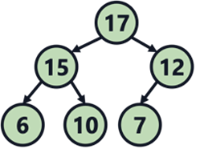
\includegraphics[width = 0.95\linewidth]{src/5_data_structure/images/max_heap.png}
    \end{minipage}
    \begin{minipage}{0.49\linewidth}
        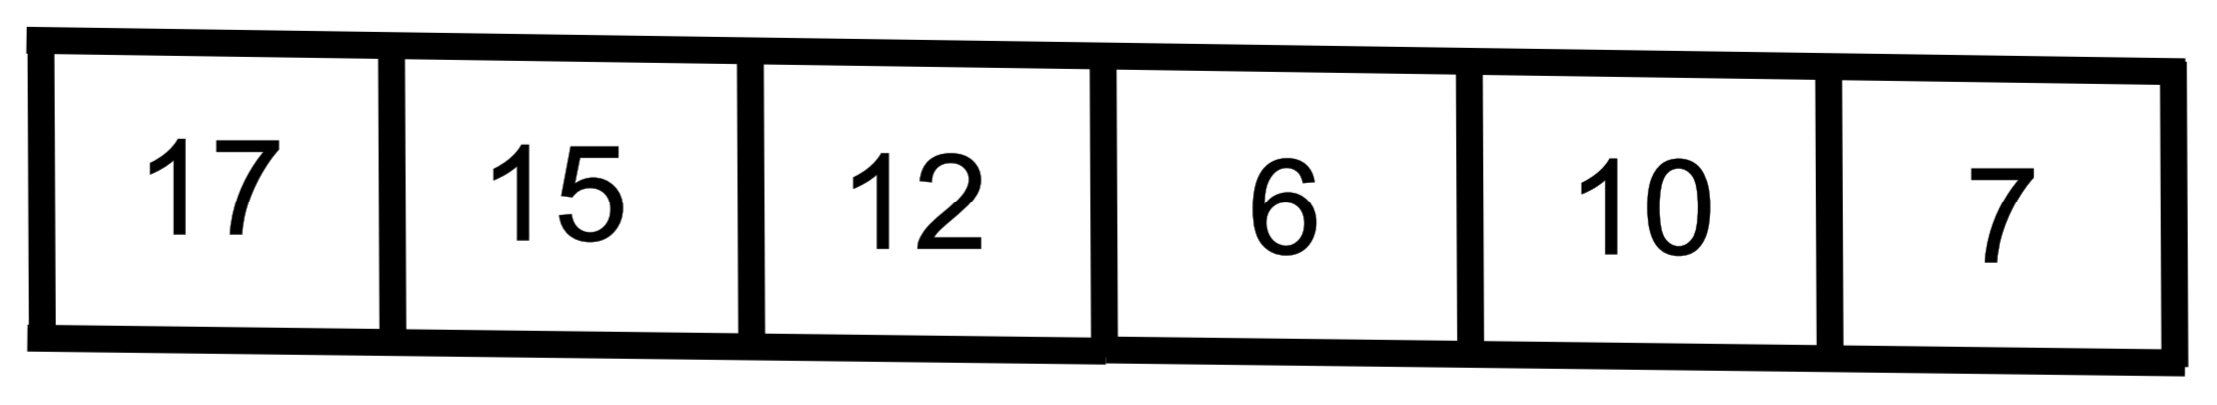
\includegraphics[width = 0.95\linewidth]{src/5_data_structure/images/max_heap_array.png}
        Array corresponding to the max heap
    \end{minipage}

    {\centering\underline{\textbf{Implementation}} \par}
        Heap[i = 1] = Root:\\
        \begin{itemize}
            \item Children of i: {2i+1, 2i+2}
            \item Parent of i: i-1//2
        \end{itemize}

    {\centering\underline{\textbf{Height}} \par}
        $H(n) = \log_2(n+1)$
        \begin{lstlisting}
# a is a heap with n elements
def height(a):
    return math.log(len(a) + 1, 2)
        \end{lstlisting}

    {\centering\underline{\textbf{Sift Up}} \par}
        Reestablishes Heap structure, Used in 'Insert'
        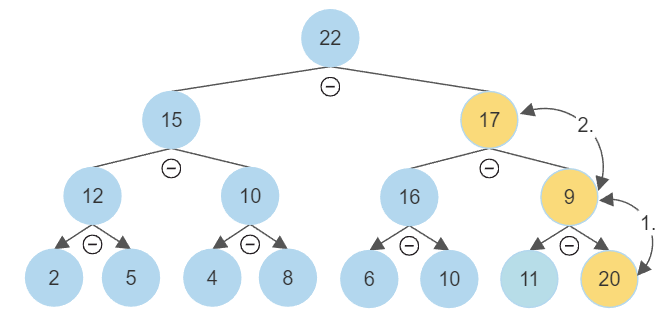
\includegraphics[width = \linewidth]{src/5_data_structure/images/heap_sift_up.png}
        \lstinputlisting{src/5_data_structure/code/heap_sift_up.py}

    {\centering\underline{\textbf{Sift Down}} \par}
        Reestablishes Heap structure, Used in 'Remove' and 'Heapify'\\
        If the parent value is smaller: exchange the parent value with the greater children value
        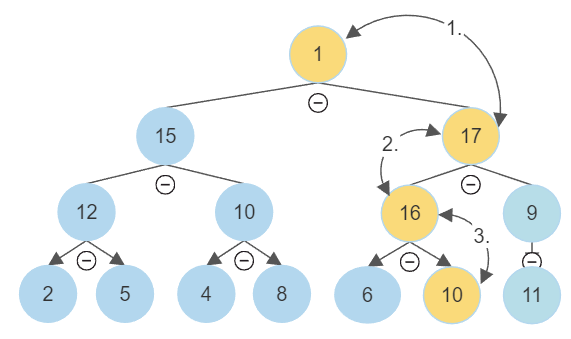
\includegraphics[width = \linewidth]{src/5_data_structure/images/heap_sift_down.png}
        \lstinputlisting{src/5_data_structure/code/heap_sift_down.py}

    {\centering\underline{\textbf{Insert}} \par}
        \lstinputlisting{src/5_data_structure/code/heap_insert.py}

    {\centering\underline{\textbf{Remove Max Value}} \par}
        Change the first and last entry in the array, then delete the last entry. Now, the max value does not exist any more.
        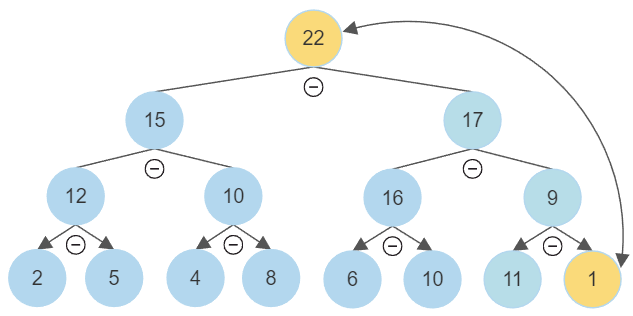
\includegraphics[width = \linewidth]{src/5_data_structure/images/heap_remove_max.png}
        Reestablish the Heap condition by applying Sift Down.
        \lstinputlisting{src/5_data_structure/code/heap_remove_max.py}

    {\centering\underline{\textbf{Heap creation / Heapify}} \par}
        Repeatedly apply Sift Down until the array is heapified.\\
        Leaves fulfill the heap condition trivially $\rightarrow$ only “heapify” the first n/2 elements.
        \lstinputlisting{src/5_data_structure/code/heap_heapify.py}

    {\centering\underline{\textbf{Sorting a heap}} \par}
        If "a" is a heap, one can efficiently sort the array:
        \lstinputlisting{src/5_data_structure/code/heap_sort.py}
    
